\section{Revis\~ao da Literatura}\label{sec:refteo}

Este capítulo apresenta uma revisão sistemática  da literatura (RSL) nos temas relacionados a previsão de séries temporais e aplicações em hidrologia e mais especificamente em abastecimento de água. A revisão bibliográfica realizada consiste em uma análise abrangente e crítica das principais fontes de literatura. As informações extraídas da literatura são fundamentais para embasar a fundamentação teórica, a metodologia e a análise dos resultados deste estudo.

Esta RSL aborda palavras chave como séries temporais, previsão, análise de séries temporais, abastecimento de água, e saneamento, que são palavras relevantes para esta pesquisa. 

A seleção das referências foi baseada em critérios específicos tais como. Definição das bases de busca, escolha das \textit{keywords}, seleção do período de busca (2016 a 2023), seleção do tipo de artigo, organização pela ordem de citações, verificação dos periódicos mais importantes (fator Q1 do Scimago e Fator de Impacto). Se um periódico pertencer ao quartil Q1 do Scimago significa que tem um desempenho melhor do que pelo menos 75\% das revistas dessa mesma categoria. Embora nem todas as referências obtidas tenham uma relação evidente ou mesmo acentuada com a área de aprendizado de máquina, elas contribuem como material de suporte a implementação de alguns modelos avaliados para previsão nesta dissertação e podem servir como base para outros estudos.

A Figura \ref{fig:serie-temporal} apresenta um fluxograma de como a pesquisa foi realizada, destacando a importância da escolha dos periódicos Q1 e com maior fator de impacto (F.I.), como base para esta RSL. A mesma figura apresenta uma adaptação da metodologia proposta por \citeonline{MARTINS201671} para a realização da RSL, onde primeiramente foram realizadas buscas na base Scopus e WoS (\textit{Web of Science}), selecionando referências relevantes para o tema da pesquisa.Para as duas bases de busca utilizadas foram usadas as palavras-chave ``\textit{time series forecasting}'', ``\textit{time series analysis}'', ``\textit{sanitation}'' e ``\textit{water supply}'' .

\begin{figure}[!htb]
	\centering
	\caption{Fluxograma da Revisão Sistemática da Literatura.}
	\label{fig:serie-temporal}
	\includegraphics[width=0.7\linewidth]{Revisao/Figuras/Figura2.pdf}
\end{figure}

Na etapa seguinte, foi realizada uma avaliação preliminar de cada artigo obtido, sem aplicar nenhum filtro anual nas buscas. Analisar todos os artigos dessa maneira resultaria em um número elevado, por exemplo, no base de dados Scopus, existiam 831 artigos, enquanto na base de dados WoS, foram encontrados 98 artigos, totalizando 929 artigos, sem a remoção de duplicatas. É importante ressaltar que esses artigos passaram apenas pelo filtro de idioma inglês e pela categoria de serem artigos (\textit{papers}), com o objetivo de aprimorar a busca e a tomada de decisões. 

Levando em consideração a diferença entre essa estimativa apresentada na Tabela \ref{tab:resumo} e a quantidade de artigos restantes após a remoção de duplicatas, tem-se menos de 929 artigos para análise. É válido lembrar que, ao remover as duplicatas, o número diminuiu ainda mais, chegando a 906 artigos.

Na etapa final, foi realizada uma análise dos conteúdos dos artigos selecionados, levando em consideração as áreas de especialização. Como esta revisão está inserida no contexto de um programa de mestrado em Engenharia de Produção e Sistemas, vale a pena analisar a relação dos artigos obtidos com áreas afins como Matemática. Assim, as áreas mais relevantes para a pesquisa foram Informática, Engenharia e Matemática, representando 50\% das publicações. 

São apresentados os resultados da RSL, utilizando um \textit{software} VOSviewer de cada base de dados utilizada no trabalho. 
A Figura \ref{fig:scopus-09-08} mostra os modelos de previsão usados com frequência em conjunto com ``\textit{time series}'' nos artigos obtidos nas bases de dados Scopus e WoS. 

\begin{figure}[!htb]
	\centering
	\caption{Modelos de previsão de series temporais na base de dados Scopus e WoS.}
	\label{fig:scopus-09-08}
	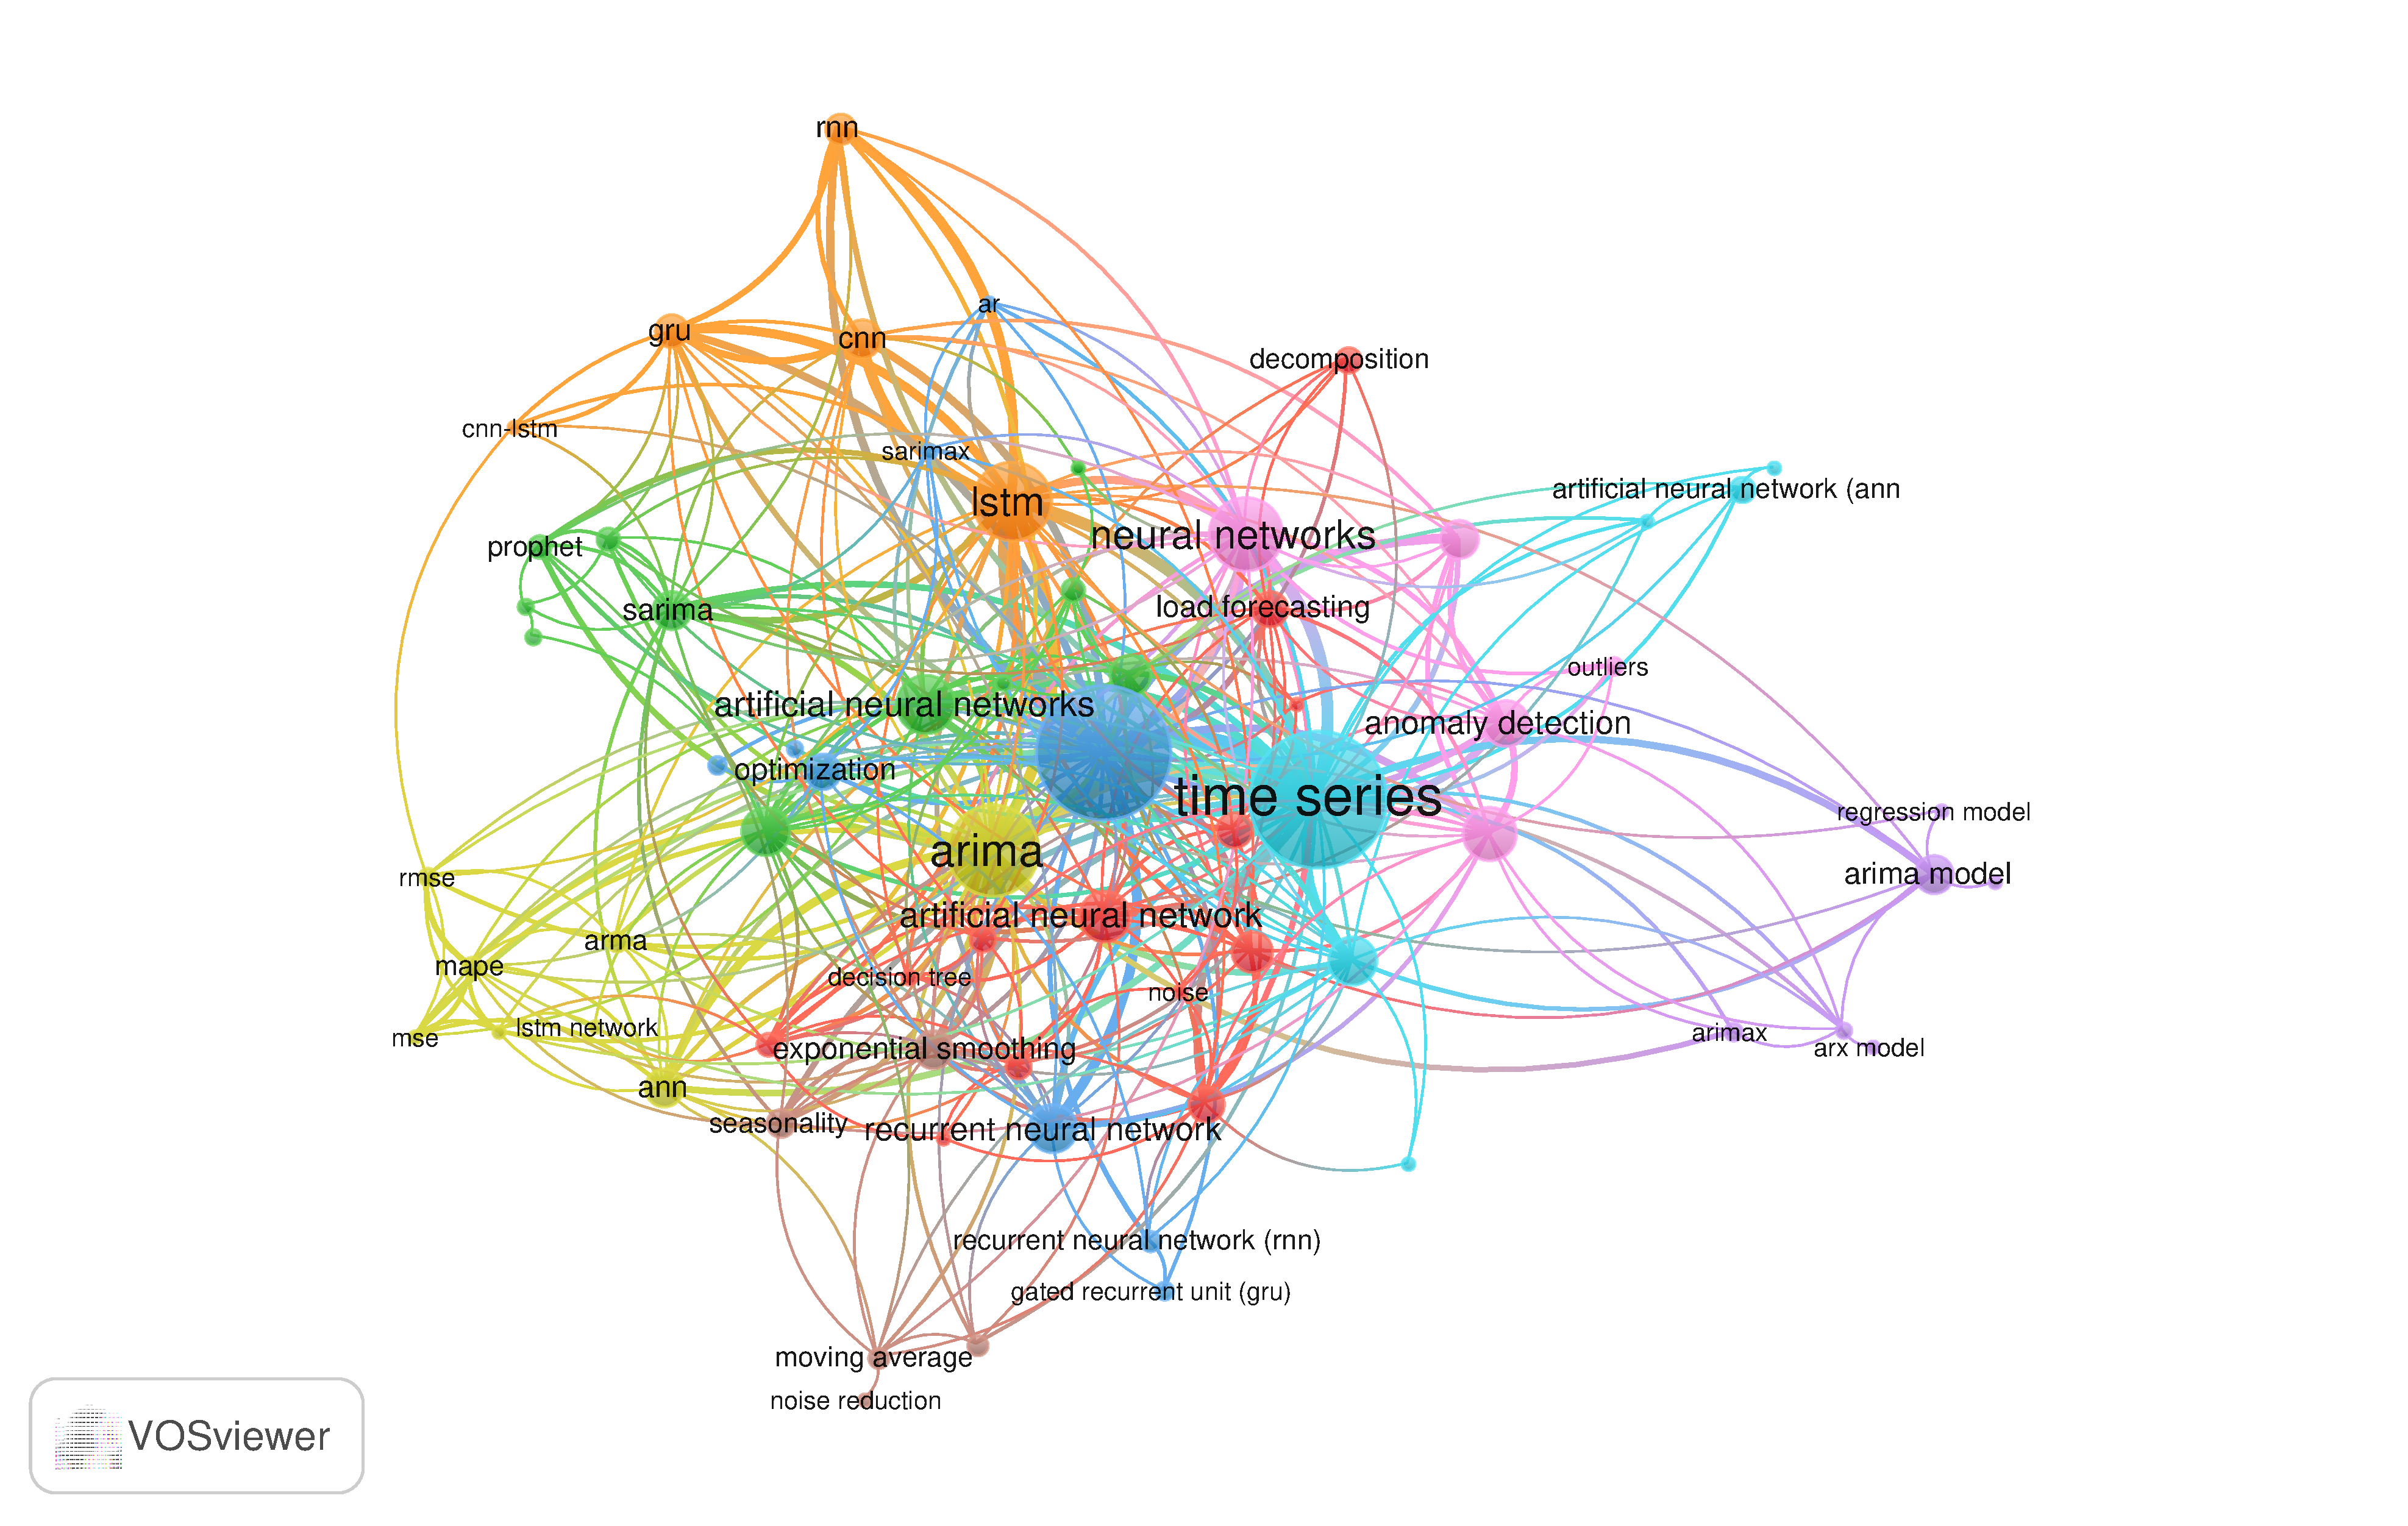
\includegraphics[width=\linewidth]{Revisao/Figuras/base-wos-scopus.pdf}
	
	
\end{figure}

Nesse primeiro momento, foram obtidos $2.555$ modelos, dos quais $83$ modelos são dispostos na Figura \ref{fig:scopus-09-08}. É importante destacar que as palavras-chave utilizadas foram \textit{time series forecasting} ou \textit{time series analysis} e \textit{water supply} e \textit{sanitation} em ambas as bases de dados. 

A Tabela \ref{tb1} apresenta as palavras-chave utilizadas em cada base de dados, juntamente com o número de artigos obtidos. No entanto, é importante ressaltar que esses dados ainda não foram processados para remover dados duplicados. Após, foi utilizado o software \textit{ScientoPy} para eliminar artigos repetidos, foram selecionados então $308$ artigos. Esses artigos foram analisados na RSL e são considerados relevantes para este estudo.

\begin{table}[!htb]
	\centering
	\caption{Combinação de palavras-chave aplicando filtros.}\label{tb1}
	\begin{tabular}{@{}lp{2cm}lp{2cm}lp{1.5cm}lp{2cm}l@{}}
		\toprule
		Bases                  & \multicolumn{7}{l}{Palavras chaves}                              & Resultados \\ \midrule
		\multirow{2}{*}{Scopus} & time series forecasting & AND & time series analysis &     &              &     &            & 798        \\
		& time series forecasting & OR  & time series analysis & AND & water supply & AND & sanitation & 33         \\
		\multirow{2}{*}{WoS}    & time series forecasting & OR  & time series analysis &     &              &     &            & 79         \\
		& time series forecasting & OR  & time series analysis & AND & water supply & AND & sanitation & 19         \\ \hline
		\multicolumn{8}{l}{Total}                                                                                              & 929        \\ \bottomrule
	\end{tabular}	
\end{table}

Na Tabela \ref{tab:resumo} são descritos os dados obtidos na RSL após a aplicação do \textit{software} \textit{ScientoPy}, onde é exibida a quantidade de artigos coletados em ambas bases Scopus e WoS. Apesar do volume considerável, os artigos não foram lidos integralmente, uma vez que muitos deles não se relacionavam diretamente com o objeto de pesquisa deste estudo. Consequentemente, ao longo da condução da RSL artigos discrepantes com o estudo foram excluídos.

\begin{table}[!htb]
	\centering
	\caption{Resumo dos artigos obtidos com a RSL nas bases Scopus e WoS.}
	\label{tab:resumo}
	\begin{tabular}{ll}
		\hline
		Quantidade de artigos obtidos & 929 \\
		Quantidade de artigos da base WoS & 98 \\
		Quantidade de artigos da base Scopus & 831 \\
		\hline
		\multicolumn{2}{c}{Remoção de artigos duplicados} \\
		\hline
		Porcentagem de artigos duplicados & 87\% \\
		Quantidade de artigos duplicados & 23 \\
		Quantidade de artigos sem duplicados & 906 \\
		Porcentagem de artigos duplicados removidos da base WoS & 19,4\% \\
		Porcentagem de artigos duplicados removidos da base Scopus & 0,5\% \\
		Quantidade de artigos duplicados com diferentes citações & 3 \\
		Porcentagem de artigos duplicados com diferentes citações & 13\% \\
		\hline
	\end{tabular}
	
\end{table}


A Tabela \ref{tb2} apresenta os periódicos onde foram publicados o maior número de artigos com as combinações utilizadas na RSL para o tema de estudo em questão. Todos os periódicos são listadas em ordem decrescente pela quantidade de publicações obtidas, incluindo a métrica do \textit{Scimago Journal Rank} (SJR) que avalia a importância relativa de periódicos científicos com base em sua influência e prestígio na comunidade acadêmica. Ele é calculado usando algoritmos complexos que levam em consideração a qualidade das citações recebidas por um periódico. Neste estudo a RSL procurou basear-se em periódicos classificados como Q1 e Q2, bem como o \textit{h-index}.

\begin{table}[!htb]
	\centering
	\caption{Classificação dos principais periódicos obtidos na RSL.}\label{tb2}
	
	\begin{tabular}{llll}		
		\toprule
		Periódicos      & No. de artigos & SJR & \textit{h-index} \\\midrule
		Neurocomputing         & 27                         & Q1                     & 143     \\
		IEEE Access            & 18                         & Q1                     & 127     \\
		Applied Soft Computing & 12                         & Q1                     & 143     \\
		Energies               & 11                         & Q2                     & 93      \\
		Energy                 & 11                         & Q1                     & 343     \\ \bottomrule
	\end{tabular}
\end{table}

O \textit{software} \textit{ScientoPy} obtém os principais tópicos de tendência com base na maior taxa de crescimento médio \textit{Average Growth Rate} (AGR). A AGR é a diferença média entre o número de documentos publicados em um ano e o número de documentos publicados no ano anterior \cite{scientopy}. Indicando como o número de documentos publicados para um tópico em específico cresceu (número positivo) ou diminuiu (número negativo) em média dentro de um período de tempo. Assim, o AGR é calculado por,

\begin{eqnarray}
	\mathrm{AGR}&=&\dfrac{\sum_{i=Y_{\mathrm{s}}}^{Y_{\mathrm{e}}} P_i-P_{i-1}}{\left(Y_{\mathrm{e}}-Y_{\mathrm{s}}\right)+1} \label{arg}
\end{eqnarray}

\noindent onde AGR é a taxa média de crescimento, $Y_e$ é o ano final, $Y_s$ é o ano inicial, $P_i$ é o número de publicações no ano $i$. Para o ano final $Y_e$, o \textit{ScientoPy} utiliza o ano final global por defeito configurado nas opções globais ou/em parâmetros do comando \textit{ScientoPy}. O ano de início $Y_s$ é calculado a partir do ano final $Y_e$, conforme calculado por,

\begin{eqnarray}
	Y_{\mathrm{s}}&=&Y_{\mathrm{e}}-(\text { WindowWidth }+1)\label{arg2}
\end{eqnarray}

\noindent onde a largura da janela (\textit{Window Width}) é predefinida como 2 anos. Assim, se o ano final for 2018, o AGR é a taxa de crescimento média entre 2017 e 2018 \cite{scientopy}.

A média de documentos por ano  \textit{Average Documents per Year} (ADY) é um indicador absoluto que representa o número médio de documentos publicados num período de tempo para um tópico específico. O ADY é calculado por,

\begin{eqnarray}
	\mathrm{ADY}&=&\dfrac{\sum_{i={Y_{\mathrm{s}}}(t)}^{Y_{\mathrm{e}}(t)} P_i}{\left(Y_{\mathrm{e}}(t)-Y_{\mathrm{s}}(t)\right)+1}\label{ady}
\end{eqnarray}

\noindent onde ADY é a média de documentos por ano, $Y_e(t)$ é o ano final, $Y_s(t)$ é o ano inicial, calculado como descrito na equação \eqref{ady}, $Pi$ é o número de publicações no ano $i$.

A porcentagem de documentos nos últimos anos  \textit{Percentage of Documents in Last Years} (PDLY) é um indicador relativo que representa a percentagem do ADY em relação ao número total de documentos para um tópico específico. Desta forma, o PDLY é calculado como,

\begin{eqnarray}
	\mathrm{PDLY}&=&\dfrac{\sum_{i={Y_{\mathrm{s}}(t)}}^{Y_{\mathrm{e}}(t)} P_i}{\left(Y_{\mathrm{e}(t)}-Y_{\mathrm{s}(t)}+1\right) \cdot \mathrm{TND}} \cdot 100 \%\label{pdly}
\end{eqnarray}

\noindent onde $PDLY$ é a percentagem de documentos nos últimos anos, $Y_e(t)$ é o ano final, $Y_s$ é o ano inicial, calculado como descrito na equação \eqref{pdly}, $P_i$ é número de publicações no ano i, $TND$ é o número total de documentos.

Tabela \ref{tb:autor} descreve os principais autores obtidos na RSL descrita previamente, sobre o tema em análise. Essa abordagem visa evitar a inclusão de todos os autores e destacar aqueles que tiveram uma contribuição significativa na área. Dessa forma, é possível identificar o principal autor que se destacou, fornecendo uma visão geral da distribuição da produção científica entre os pesquisadores. Na Tabela \ref{tb:autor} são descritos os valores da taxa de crescimento médio AGR, documentos médios por ano ADY, e porcentagem de documentos nos últimos anos PDLY no período de 2021 a 2023.

\begin{table}[!htb]
	\centering
	\caption{Total de publicações dos principais autores obtidos na RSL.}\label{tb:autor}
	\begin{tabular}{llllll}
		\hline
		Author & No. de artigos & AGR & ADY & PDLY & \textit{h-index} \\
		\hline
		\citeonline{2-s2.0-84973369468} & 11 & $-0,5$ & 2 & 36,4 & 8 \\
		\citeonline{2-s2.0-85123707840} & 11 & 0 & 3 & 54,5 & 5 \\
		\citeonline{2-s2.0-85018469706} & 10 & 1 & 2,5 & 50 & 5 \\
		\citeonline{2-s2.0-85048003524} & 9 & $-1,5$ & 2 & 44,4 & 4 \\
		\citeonline{2-s2.0-84964575877} & 7 & 1,5 & 2 & 57,1 & 3 \\
		\citeonline{2-s2.0-85063200888} & 7 & 1 & 2 & 57,1 & 3 \\
		\citeonline{2-s2.0-85148656225} & 7 & 1 & 3 & 85,7 & 2 \\
		\citeonline{2-s2.0-85041536076} & 7 & 1,5 & 3 & 85,7 & 3 \\
		\citeonline{2-s2.0-85130875471} & 6 & 0 & 1,5 & 50 & 4 \\
		\citeonline{2-s2.0-85061810603} & 6 & 0 & 1,5 & 50 & 5 \\
		\hline
	\end{tabular}
\end{table}



A Tabela \ref{tb:pais} apresenta os países com maior número de artigos obtidos na RSL usando as palavras-chaves citadas previamente. Tais países estão ordenados de forma decrescente pelo número de publicações obtido. Os principais países que se destacam nessa análise são China, com $179$ publicações, Estados Unidos da América com $74$ publicações, Índia com $61$ publicações, Brasil com $49$ publicações, Espanha com $40$ publicações, Reino Unido com $40$ publicações, Austrália com $31$ publicações, Itália com $26$ publicações, Canadá com $25$, Irã com $20$ publicações.

\begin{table}[!htb]
	\centering
	\caption{Total de publicações dos principais países obtidos na RSL.}\label{tb:pais}
	\begin{tabular}{llllll}
		\toprule
		País & No. de artigos & AGR & ADY & PDLY & \textit{h-index} \\
		\midrule
		China & 179 & 18,5 & 48 & 53,6 & 31 \\
		Estados Unidos da América & 74 & 3 & 16 & 43,2 & 21 \\
		Índia & 61 & 0 & 12 & 39,3 & 18 \\
		Brasil & 49 & 3,5 & 12,5 & 51 & 17 \\
		Espanha & 40 & 1,5 & 8,5 & 42,5 & 12 \\
		Reino Unido & 40 & 3 & 10 & 50 & 15 \\
		Austrália & 31 & 3,5 & 7,5 & 48,4 & 14 \\
		Itália & 26 & 2 & 7 & 53,8 & 10 \\
		Canadá & 25 & 1 & 5,5 & 44 & 11 \\
		Irã & 20 & $-1$ & 3,5 & 35 & 11 \\
		\bottomrule
	\end{tabular}
\end{table}



Foi realizada uma análise dos artigos obtidos com a RSL. Esses artigos retratam alguns dos modelos de previsão utilizados em 
\citeonline{Taieb2016, Ursu2016, Wang2016, Graff2017, Tyralis2017, Boroojeni2017, Coelho2017, Chou2018, Bergmeir2018, Rossi2018, Ahmad2018, Chou2018a, Chen2018, Sadaei2019, Yang2019a, Buyuksahin2019, CarvalhoJr.2019, Liu2019, Shih2019a, Moon2019, Yang2019a, Xu2019, Golyandina2020, Martinovic2020a, Salgotra2020, Vlachas2020, Kulshreshtha2020, Samanta2020, Shen2020, Sezer2020, Du2020, Li2020,  Kumar2021, Lara-Benitez2021, Tan2021, Liu2021}.

Notou-se que em tais artigos diferentes modelos de previsão de séries temporais foram utilizados. Eles representam contribuições significativas para o avanço do conhecimento e aplicação prática das séries temporais, sobre abordagens eficazes nesse campo. 

Por exemplo, no estudo conduzido por \citeonline{Xu2019}, um modelo híbrido foi proposto, combinando o modelo linear AR e LR com o modelo não-linear ARIMA e o modelo \textit{Dynamic Bayesian Network} (DBN) . Essa abordagem permitiu capturar tanto os comportamentos lineares quanto os não-lineares de uma série temporal. 

Por outro lado, \citeonline{Li2020} comparou o desempenho de previsão da abordagem MAELS (Modelo Alternativo de Estação Livre Série Temporal) com outros modelos de aprendizado de máquina como CNN, RNN, LSTM, GRU, Transformer, Prophet, ARIMA e \textit{Support Vector Machine Variable Regression} (SVM-VAR) . As abordagens CNN, RNN, GRU, Transformer e LSTM foram capazes de trabalhar com dados multivariados de entrada e saída, enquanto o ARIMA utiliza informações passadas para prever o futuro com base em características como autocorrelação e médias móveis. 

Na Tabela \ref{tb:mode} é apresentada a quantidade de artigos foram obtidos pela RSL para cada modelo de previsão e também cita-se pelo menos um autor correspondente a cada modelo.

\begin{table}[!htb]
	\centering
	\caption{Principais modelos de previsão obtidos na RSL.}\label{tb:mode}
	\small % Utilize uma fonte menor
	\begin{tabular}{lllllll}
		\toprule
		Modelos & Autores & No. & AGR & ADY & PDLY & \textit{h-index} \\
		\midrule
		ARX & \citeonline{2-s2.0-85051469381} & 3 & 0 & 0,7 & 66,7 & 2 \\	
		ARMA & \citeonline{2-s2.0-85038637324} & 7 & 0,3 & 0,7 & 28,6 & 6 \\
		ARIMA & \citeonline{2-s2.0-85069459067} & 84 & 1,7 & 16,7 & 59,5 & 27 \\
		SARIMA & \citeonline{2-s2.0-85128561644} & 5 & 1 & 1,7 & 100 & 4 \\
		SARIMAX & \citeonline{2-s2.0-85099424908} & 2 & 0,3 & 0,7 & 100 & 2 \\	
		LSTM & \citeonline{WOS:000529902300014} & 35 & 3,3 & 10,7 & 91,4 & 16 \\
		RNN & \citeonline{2-s2.0-85067419084} & 20 & 0 & 4,3 & 65 & 11 \\
		Árvores de Decisão & \citeonline{2-s2.0-85054695177} & 12 & 0,7 & 3 & 75 & 7 \\
		RF & \citeonline{2-s2.0-85135210428} & 9 & 1,7 & 2,7 & 88,9 & 5 \\
		CNN & \citeonline{WOS:000841076700002} & 8 & 1,3 & 2,7 & 100 & 4 \\
		GRU & \citeonline{2-s2.0-85135210428} & 5 & 0 & 1,3 & 80 & 4 \\
		LR & \citeonline{2-s2.0-85125426780} & 3 & 0 & 0,7 & 66,7 & 3 \\
		Prophet & \citeonline{2-s2.0-85092514286} & 3 & 0,3 & 1 & 100 & 3 \\
		XGBoost & \citeonline{2-s2.0-85130441623} & 1 & 0,3 & 0,3 & 100 & 0 \\
		\bottomrule
	\end{tabular}
\end{table}

Além dos modelos prévios, também será utilizada a versão atualizada do ARIMA nesta dissertação, bem como os modelos SARIMA e SARIMAX serão comparados para determinar qual deles é o mais adequado. Além disso, serão empregados os modelos Light GBM e XGBoost. Os modelos de aprendizado profundo, como a RNN, ainda é considerada um excelente modelo para previsão de séries temporais no tema de saneamento básico que está estudado.

Embora existam várias ramificações do modelo ARIMA, o modelo desenvolvido pelo Facebook, conhecido como Prophet, sobressai como uma opção superior em comparação com os demais. O Prophet é um modelo mais recente que simplifica significativamente muitas das tarefas que são necessárias ao lidar com o ARIMA. Enquanto o Prophet foi criado em 2017, o modelo ARIMA tem relatos de ter sido desenvolvido na década de 1960. Essa diferença temporal destaca a evolução e a modernização do campo de modelagem de séries temporais ao longo das décadas \cite{ramos2010previsoes}.
